\documentclass[10pt]{article}
\usepackage[pdftex]{graphicx, color}
\usepackage{listings,proof}

\usepackage{tikz}
\usepackage{hyperref}
\usetikzlibrary{automata,positioning}

\headheight 8pt \headsep 20pt \footskip 30pt
\textheight 9in \textwidth 6.5in
\oddsidemargin 0in \evensidemargin 0in
\topmargin -.35in
\lstset{
  basicstyle=\ttfamily,
  mathescape
}
\lstset{basicstyle=\small\ttfamily,breaklines=true}
\newcommand {\pts}[1]{{\bf #1 pts}}
\newcommand{\ttmath}[1]{$\mathtt{#1}$}
\newcommand{\ossimple}[6]{#1,#2,#3\vdash #4 : #5,#6}
\newcommand{\osrule}[8]{\frac{#7}{\ossimple{#1}{#2}{#3}{#4}{#5}{#6}}\eqno
  \mbox{#8}}
\newcommand{\infertext}[2]{\infer{{\textrm{#1}}}{#2}}

\begin{document}
\begin{center}
    \Large CS131 Compilers: Writing Assignment 3\\
    Due Sunday, May 1, 2022 at 23:59pm
\end{center}

\begin{center}
    %% Change this:
    \LARGE Tian Haoyuan - 2020533013
\end{center}

This assignment asks you to prepare written answers to questions on
semantic analysis. Each of the questions has a short answer. You
may discuss this assignment with other students and work on the problems
together. However, your write-up should be your own individual work.
and you should indicate in your submission who you worked with, if applicable.
Written assignments are turned in at the start of lecture.
You should use the Latex template provided at the course web site to write your solution.

\begin{center}
    %% Change this:
    I worked with: nobody
\end{center}

Example for type rule in tex:
\[\infertext
    {$O$[Bo/x][Ob/x] $\vdash$ x: Ob}
    {\textrm{$O$[Bo/x][Ob/x](x) = Ob}}
\]
\begin{enumerate}
    \item (4x2 pts) \textbf{3-AC.} a = b*(minus c) + b*(minus c)
          \begin{itemize}
              \item Give 3-address code.
              \item Give quadruples table.
              \item Give triples table.
              \item Give indirect triples table.
          \end{itemize}
          \textcolor{blue}{
              \begin{itemize}
                  \item $t_1=minus\ c\\t_2=b*t_1\\t_3=minua\ c\\t_4=b*t_3\\a=t_2+t_4\\a=t_5$
                  \item
                        \begin{tabular}{c|l|c|c|c}
                                & op    & result & arg1  & arg2  \\
                            \hline
                            (1) & minus & $t_1$  & c             \\
                            (2) & *     & $t_2$  & b     & $t_1$ \\
                            (3) & minus & $t_3$  & c             \\
                            (4) & *     & $t_4$  & b     & $t_3$ \\
                            (5) & +     & $t_5$  & $t_2$ & $t_4$ \\
                            (6) & =     & a      & $t_5$ &
                        \end{tabular}
                  \item
                        \begin{tabular}{c|l|c|c}
                                & op    & arg1 & arg2 \\
                            \hline
                            \hline
                            (1) & minus & c           \\
                            (2) & *     & b    & (1)  \\
                            (3) & minus & c           \\
                            (4) & *     & b    & (3)  \\
                            (5) & +     & (2)  & (4)  \\
                            (6) & =     & a    & (5)
                        \end{tabular}
                  \item
                        \begin{tabular}{|c|c|}
                            \hline
                            (1) & (11) \\
                            \hline
                            (2) & (12) \\
                            \hline
                            (3) & (13) \\
                            \hline
                            (4) & (14) \\
                            \hline
                            (5) & (15) \\
                            \hline
                            (6) & (16) \\
                            \hline
                        \end{tabular}
                        \begin{tabular}{c|l|c|c}
                                 & op    & arg1 & arg2 \\
                            \hline
                            \hline
                            (11) & minus & c           \\
                            (12) & *     & b    & (11) \\
                            (13) & minus & c           \\
                            (14) & *     & b    & (13) \\
                            (15) & +     & (12) & (14) \\
                            (16) & =     & a    & (15)
                        \end{tabular}
              \end{itemize}
          }
    \item (2x4 pts) \textbf{SDD.}
          \begin{enumerate}
              \item Given Syntax-Directed Definition below construct the annotated parse tree for the input express "int a,
                    b, c".
                    \begin{table}[h]
                        \centering
                        \begin{tabular}{ll}
                            D $\rightarrow$ TL          & L.inh = T.type           \\
                            T $\rightarrow$ int         & T.type = integer         \\
                            T $\rightarrow$ float       & T.type = float           \\
                            L $\rightarrow$ $L_{1}$, id & $L_{1}$.inh = L.inh      \\
                                                        & addType(id.entry, L.inh) \\
                            $L_1$ $\rightarrow$ id      & addType(id.entry, L.inh)
                        \end{tabular}
                    \end{table}
                    \textcolor{blue}{
                        \begin{center}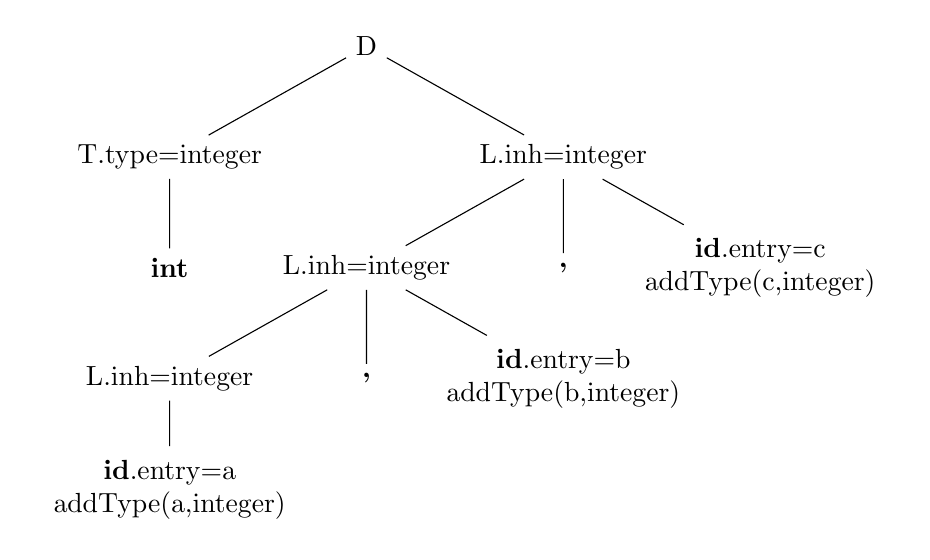
\begin{tikzpicture}    [
                                    level distance = 4em,
                                    level 1/.style={sibling distance=5cm},
                                    level 2/.style={sibling distance=2.5cm},
                                    level 3/.style={sibling distance=2.5cm}
                                ]
                                \node(root){D}
                                child{node{T.type=integer}
                                        child{node{\textbf{int}}}
                                    }
                                child{node{L.inh=integer}
                                        child{node{L.inh=integer}
                                                child{node{L.inh=integer}
                                                        child{node{\begin{tabular}{c}
                                                                            \textbf{id}.entry=a \\
                                                                            addType(a,integer)
                                                                        \end{tabular}}}}
                                                child{node{\textbf{,}}}
                                                child{node{\begin{tabular}{c}
                                                                    \textbf{id}.entry=b \\
                                                                    addType(b,integer)
                                                                \end{tabular}}}
                                            }
                                        child{node{\textbf{,}}}
                                        child{node{
                                                        \begin{tabular}{c}
                                                            \textbf{id}.entry=c \\
                                                            addType(c,integer)
                                                        \end{tabular}
                                                    }}
                                    };
                            \end{tikzpicture}\end{center}
                    }
              \item Given the Syntax-Directed Definition below with the synthesized attribute $val$, draw the annotated
                    parse tree for the express "(7 + 8)*(9 + 10)".
                    \begin{table}[h]
                        \centering
                        \begin{tabular}{ll}
                            L $\rightarrow$ E           & L.val = E.val               \\
                            E $\rightarrow$ T           & E.val = T.val               \\
                            E $\rightarrow$ $E_{1}$ + T & E.val = $E_{1}$.val + T.val \\
                            T $\rightarrow$ F           & T.val = F.val               \\
                            T $\rightarrow$ $T_{1}$ * F & T.val = $T_{1}$.val * F.val \\
                            F $\rightarrow$ (E)         & F.val = E.val               \\
                            F $\rightarrow$ digit       & F.val = digit.lexval
                        \end{tabular}
                    \end{table}
                    \textcolor{blue}{
                        \begin{center}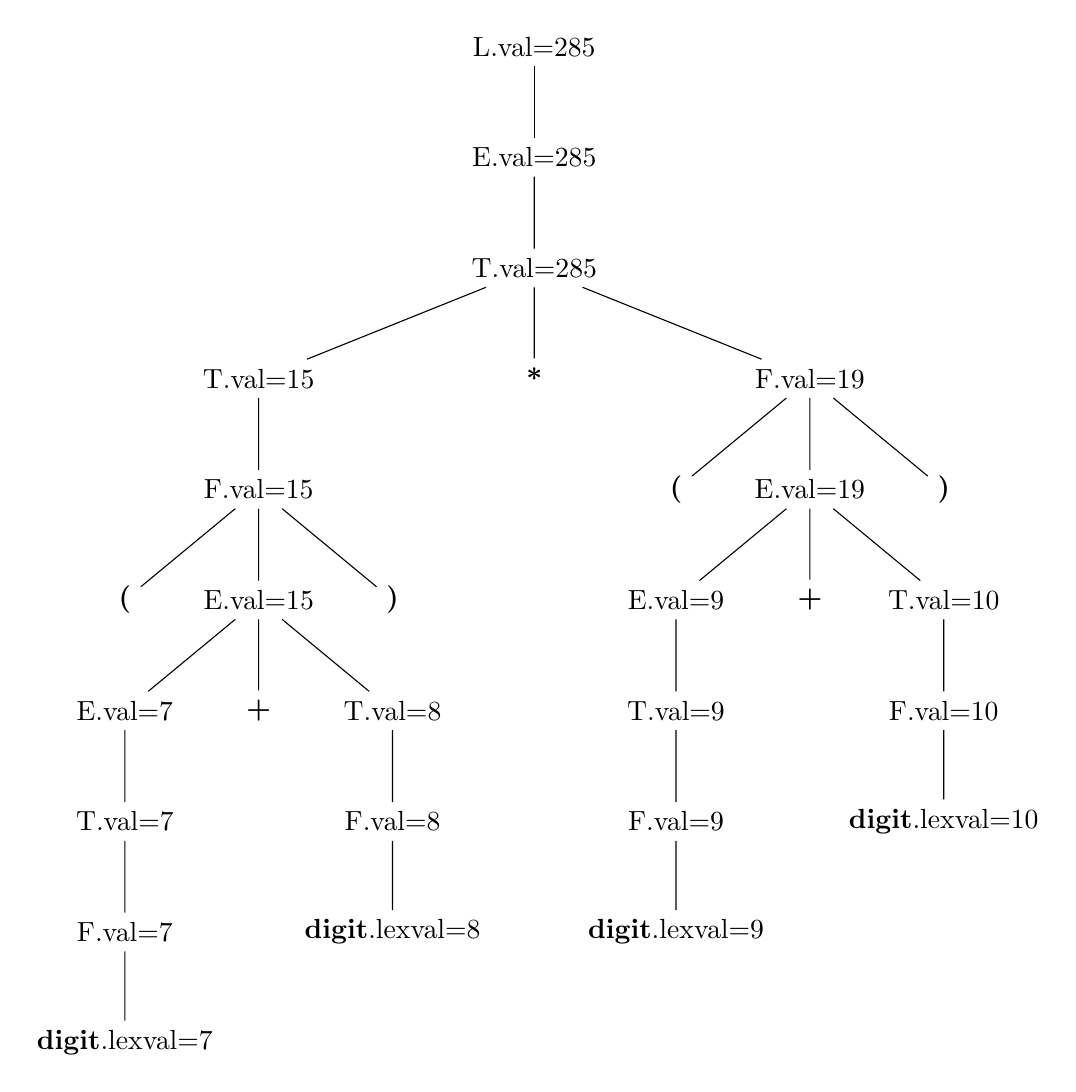
\begin{tikzpicture}    [
                                    level distance = 4em,
                                    level 1/.style={sibling distance=5cm},
                                    level 2/.style={sibling distance=1.5cm},
                                    level 3/.style={sibling distance=3.5cm},
                                    level 4/.style={sibling distance=1.7cm},
                                ]
                                \node(root){L.val=285}
                                child{node{E.val=285}
                                        child{node{T.val=285}
                                                child{node{T.val=15}
                                                        child{node{F.val=15}
                                                                child{node{\textbf{(}}}
                                                                child{node{E.val=15}
                                                                        child{node{E.val=7}
                                                                                child{node{T.val=7}
                                                                                        child{node{F.val=7}
                                                                                                child{node{\textbf{digit}.lexval=7}
                                                                                                    }
                                                                                            }
                                                                                    }
                                                                            }
                                                                        child{node{\textbf{+}}
                                                                            }
                                                                        child{node{T.val=8}
                                                                                child{node{F.val=8}
                                                                                        child{node{\textbf{digit}.lexval=8}
                                                                                            }
                                                                                    }
                                                                            }
                                                                    }
                                                                child{node{\textbf{)}}}
                                                            }
                                                    }
                                                child{node{\textbf{*}}
                                                    }
                                                child{node{F.val=19}
                                                        child{node{\textbf{(}}}
                                                        child{node{E.val=19}
                                                                child{node{E.val=9}
                                                                        child{node{T.val=9}
                                                                                child{node{F.val=9}
                                                                                        child{node{\textbf{digit}.lexval=9}
                                                                                            }
                                                                                    }
                                                                            }
                                                                    }
                                                                child{node{\textbf{+}}
                                                                    }
                                                                child{node{T.val=10}
                                                                        child{node{F.val=10}
                                                                                child{node{\textbf{digit}.lexval=10}
                                                                                    }
                                                                            }
                                                                    }
                                                            }
                                                        child{node{\textbf{)}}}
                                                    }
                                            }
                                    }
                                ;
                            \end{tikzpicture}\end{center}
                    }
          \end{enumerate}
    \item (4x2 pts) \textbf{SDD.} Construct a Syntax-Directed Translation scheme that takes strings of a's, b's
          and c's as input and produces as output the number of substrings in the input string tha correspond to the pattern
          a(a|b)*c+(a|b)*b. For example the translation of the input string "abbcabcababc" is 3 ("abbcab", "abcab",
          "abcabab").\\
          \begin{itemize}
              \item Create a CFG that generates all string of a's, b's and c's.\\
                    \textcolor{blue}{
                        The CFG: $G=\{\{a,b,c\},\{S\},S,P\}$, where the production law $P$ is as follows.
                        \[\begin{array}{cll}
                                %% Your answer here
                                S & \rightarrow & Sa \\
                                S & \rightarrow & Sb \\
                                S & \rightarrow & Sc \\
                                S & \rightarrow & a  \\
                                S & \rightarrow & b  \\
                                S & \rightarrow & c
                            \end{array}\]
                    }
              \item Semantic attributes for the grammar symbols.\\
                    \textcolor{blue}{
                        Define 3 synthesized attributes for S:\\
                        count\_a, which accumulates the number of 'a's that are left to a given 'c';\\
                        keep\_a, which keeps the number of 'a's that were left to a given 'c';\\
                        acc, which counts the number substrings that satisfy the requirement.\\
                        Explanation:\\
                        In a substring under consideration, since only the number of 'a' matter before a given 'c', so we keep track on the nunmber of 'a' with count\_a; after a given 'c' in a substring, only the number of 'b' matters, by multiplying the number of 'a' before that c, so it is necessary to keep the number of 'a' in another attribute keep\_a, since count\_a would turn to count the number of 'a' for next 'c'.
                    }
              \item For each production of the grammar a set of rules for evaluation of the semantic attributes.
                    \textcolor{blue}{
                        \[\begin{array}{clll}
                                %% Your answer here
                                S & \rightarrow & S_1a & \{S.count\_a=S_1.count\_a+1;S.keep\_a=S_1.keep\_a;S.acc=S_1.acc;\}           \\
                                S & \rightarrow & S_1b & \{S.count\_a=S_1.count\_a;S.keep\_a=S_1.keep\_a;S.acc=S_1.acc+S_1.keep\_a;\} \\
                                S & \rightarrow & S_1c & \{S.count\_a=0;S.keep\_a=S_1.count\_a;S.acc=S_1.acc;\}                       \\
                                S & \rightarrow & a    & \{S.count\_a=1;S.keep\_a=0;S.acc=0;\}                                        \\
                                S & \rightarrow & b    & \{S.count\_a=0;S.keep\_a=0;S.acc=0;\}                                        \\
                                S & \rightarrow & c    & \{S.count\_a=0;S.keep\_a=0;S.acc=0;\}
                            \end{array}\]
                    }
              \item Justification that your solution is correct.\\
                    \textcolor{blue}{
                        Here's the annotated parse tree of string "abbcabcababc".
                        \begin{center}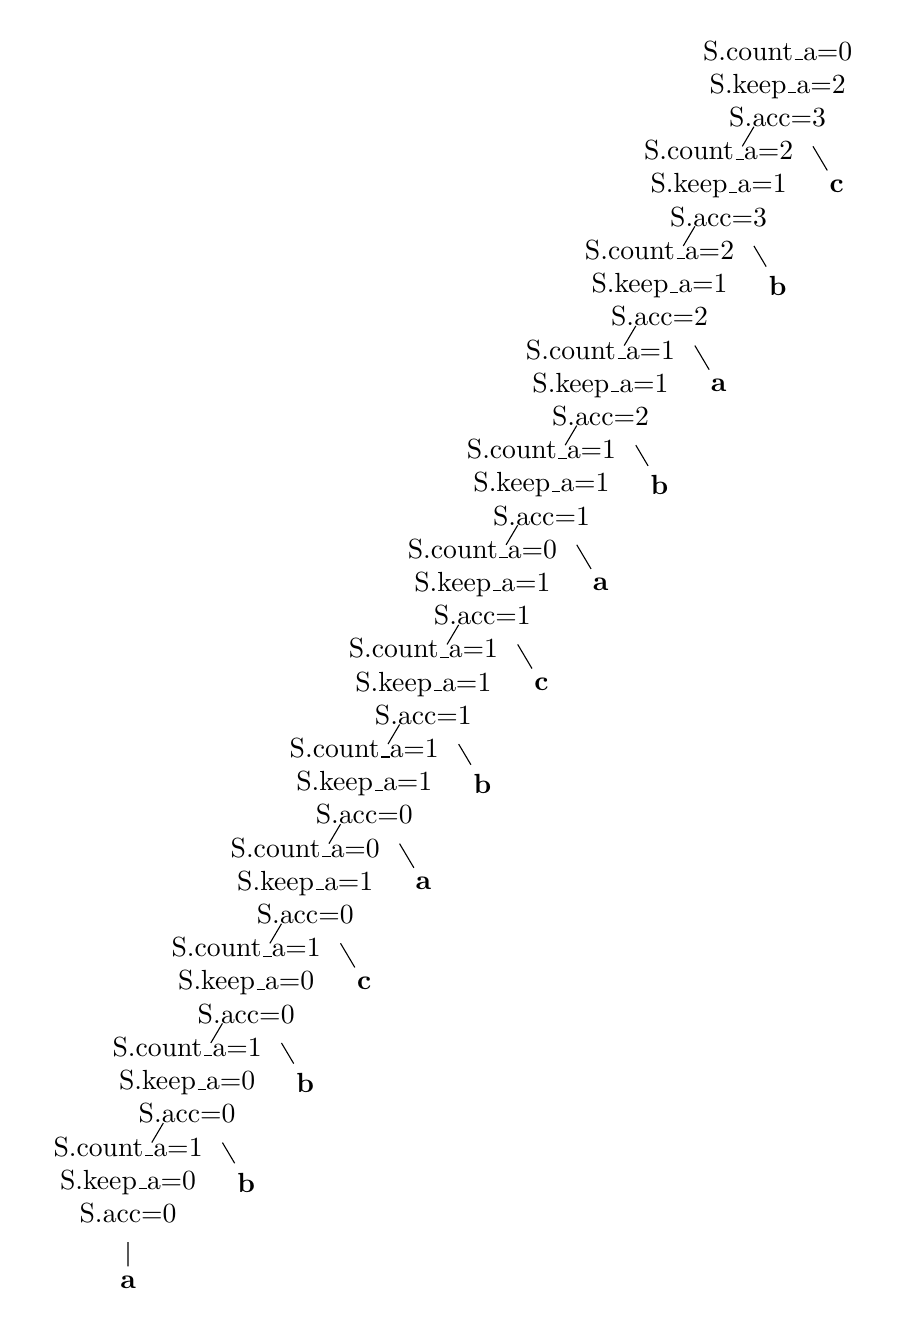
\begin{tikzpicture}    [
                                    level distance = 3.6em,
                                    level 1/.style={sibling distance=1.5cm},
                                    level 2/.style={sibling distance=1.5cm},
                                    level 3/.style={sibling distance=1.5cm}
                                ]
                                \node(root){\begin{tabular}{c}
                                        S.count\_a=0 \\
                                        S.keep\_a=2  \\
                                        S.acc=3
                                    \end{tabular}}
                                child{node{\begin{tabular}{c}
                                            S.count\_a=2 \\
                                            S.keep\_a=1  \\
                                            S.acc=3
                                        \end{tabular}
                                    }
                                child{node{\begin{tabular}{c}
                                            S.count\_a=2 \\
                                            S.keep\_a=1  \\
                                            S.acc=2
                                        \end{tabular}
                                    }child{node{\begin{tabular}{c}
                                            S.count\_a=1 \\
                                            S.keep\_a=1  \\
                                            S.acc=2
                                        \end{tabular}
                                    }child{node{\begin{tabular}{c}
                                            S.count\_a=1 \\
                                            S.keep\_a=1  \\
                                            S.acc=1
                                        \end{tabular}
                                    }child{node{\begin{tabular}{c}
                                            S.count\_a=0 \\
                                            S.keep\_a=1  \\
                                            S.acc=1
                                        \end{tabular}
                                    }child{node{\begin{tabular}{c}
                                            S.count\_a=1 \\
                                            S.keep\_a=1  \\
                                            S.acc=1
                                        \end{tabular}
                                    }child{node{\begin{tabular}{c}
                                            S.count\_a=1 \\
                                            S.keep\_a=1  \\
                                            S.acc=0
                                        \end{tabular}
                                    }child{node{\begin{tabular}{c}
                                            S.count\_a=0 \\
                                            S.keep\_a=1  \\
                                            S.acc=0
                                        \end{tabular}
                                    }child{node{\begin{tabular}{c}
                                            S.count\_a=1 \\
                                            S.keep\_a=0  \\
                                            S.acc=0
                                        \end{tabular}
                                    }child{node{\begin{tabular}{c}
                                            S.count\_a=1 \\
                                            S.keep\_a=0  \\
                                            S.acc=0
                                        \end{tabular}
                                    }child{node{\begin{tabular}{c}
                                            S.count\_a=1 \\
                                            S.keep\_a=0  \\
                                            S.acc=0
                                        \end{tabular}
                                    }
                                child{node{\textbf{a}}}
                                }
                                child{node{\textbf{b}}}
                                }
                                child{node{\textbf{b}}}
                                }
                                child{node{\textbf{c}}}
                                }
                                child{node{\textbf{a}}}
                                }
                                child{node{\textbf{b}}}
                                }
                                child{node{\textbf{c}}}
                                }
                                child{node{\textbf{a}}}
                                }
                                child{node{\textbf{b}}}
                                }
                                child{node{\textbf{a}}}
                                }
                                child{node{\textbf{b}}}
                                }
                                child{node{\textbf{c}}};
                            \end{tikzpicture}\end{center}
                        Since $S.count\_a$ counts the number of 'a' of the substring under consideration, and when it encounters 'c', we start to count for the next substring instead of the last one, and we save the number of 'a' to $S.keep\_a$ as a constant. Each time it encounters a 'b', we can find $1\times S.keep\_a$ substrings that satisfy the requirement. So, keeping an eye on each 'b' in the whole string, which appears as an end of a qualified substring, we can find all of these substrings, that is "abbcab", "abcab", "abcabab".
                    }
          \end{itemize}
    \item (3x4 pts) \textbf{Type checking.} Give the Semantic Rule.  All the attributes are synthesized.
          \begin{itemize}
              \item The syntax directed definition for associating a type to an Expression if $num$ stands for an
                    integer number. $\uparrow$ means pointer.
                    \begin{table}[h]
                        \centering
                        \begin{tabular}{l}
                            E $\rightarrow$ num $\big|$ id $\big|$  E mod E $\big|$ E{[}E{]} $\big|$ E $\uparrow$
                        \end{tabular}
                    \end{table}

                    \textcolor{blue}{\\
                        \begin{tabular}{ll}
                            $E \rightarrow num$           & \{ $E.type=integer; $\}          \\
                            $E \rightarrow id$            & \{ $E.type=loopup(id.entry); $\} \\
                            $E \rightarrow E_1\ mod\ E_2$ & \begin{tabular}{ll}
                                \{ & if( $E_1.type==integer\ \&\&\ E_2.type==integer$ ) \\
                                   & \{ $E.type=integer$; \}                            \\
                                   & else\{ E.type = type\_error; \} \}
                            \end{tabular}       \\
                            $E \rightarrow E_1[E_2]$      & \begin{tabular}{ll}
                                \{ & if( $E_1.type==array(s,t)\ \&\&\ E_2.type==integer$ ) \\
                                   & \{ $E.type=t$; \}                                     \\
                                   & else\{ E.type = type\_error; \} \}
                            \end{tabular}       \\
                            $E \rightarrow E_1\uparrow$   & \begin{tabular}{ll}
                                \{ & if( $E_1.type==pointer(t)$ )       \\
                                   & \{ $E.type=t$; \}                  \\
                                   & else\{ E.type = type\_error; \} \}
                            \end{tabular}       \\
                        \end{tabular}
                    }
              \item The syntax directed definition for associating a type to a Statement. $E$ is the expression in 5.1.
                    \begin{table}[h]
                        \centering
                        \begin{tabular}{l}
                            S $\rightarrow$ id := E $\big|$ if E then S $\big|$ while E do S $\big|$ S; S
                        \end{tabular}
                    \end{table}
                    \textcolor{blue}{\\
                        \begin{tabular}{ll}
                            $S \rightarrow id:=E$            & \{ if( $id.type==E.type$ ) \{ $S.type=void$; \} else \{ S.type = type\_error; \} \}           \\
                            $S \rightarrow if\ E\ then\ S1$  & \{ if( $E.type==Bool $) \{ $S.type=S_1.type$; \} else \{ S.type = type\_error; \} \}          \\
                            $S \rightarrow while\ E\ do\ S1$ & \{ if( $E.type==Bool $) \{ $S.type=S_1.type$; \} else \{ S.type = type\_error; \} \}          \\
                            $S \rightarrow S_1;S_2$          & \{if( $S_1.type==void\ \&\& S_2.type==void$)\{$S.type=void$;\}else\{S.type = type\_error;\}\} \\
                        \end{tabular}
                    }
              \item The syntax directed definition for associating a type to a function.
                    \begin{table}[h]
                        \centering
                        \begin{tabular}{l}
                            F $\rightarrow$ fun id(D): T; B                                          \\
                            D $\rightarrow$ id: T $\big|$ D; D                                       \\
                            T $\rightarrow$ char $\big|$  int $\big|$  array{[}num{]} of T $\big|$ T \\
                            B $\rightarrow$ \{S\}                                                    \\
                            S $\rightarrow$ id(EList)                                                \\
                            EList $\rightarrow$ E $\big|$  Elist, E
                        \end{tabular}
                    \end{table}
                    \textcolor{blue}{\\
                        \begin{tabular}{ll}
                            $F \rightarrow fun\ id(D):T;B$      & \{ $id.type=D.type\rightarrow T.type$; \}                                                         \\
                            $D \rightarrow id:T$                & \{ $D.type=T.type;\ addType(id.entry,T.type)$; \}                                                 \\
                            $D \rightarrow D_1;D_2$             & \{ $D.type=D_1.type\times D_2.type$; \}                                                           \\
                            $T \rightarrow char$                & \{ $T.type=char$; \}                                                                              \\
                            $T \rightarrow int$                 & \{ $T.type=int$; \}                                                                               \\
                            $T \rightarrow array[num]\ of\ T_1$ & \{ $T.type=list(T_1.type)$; \}                                                                    \\
                            $T \rightarrow T_1$                 & \{ $T.type=T_1.type$; \}                                                                          \\
                            $B \rightarrow \{S\}$               &                                                                                                   \\
                            $S \rightarrow id(Elist)$           & \{if($Elist.type==s\ \&\&\ id.type=s\rightarrow t$)\{$S.type=t$;\}else\{$S.type=type\_error$;\}\} \\
                            $Elist \rightarrow E$               & \{ $Elist.type=E.type$; \}                                                                        \\
                            $Elist \rightarrow Elist_1,E$       & \{ $Elist.type=Elist_1.type\times E.type$; \}                                                     \\
                        \end{tabular}
                    }
          \end{itemize}

    \item (10 pts) \textbf{Type Inference.} Consider the following class definitions.
          \begin{verbatim}
  class A {
    i: Int
    o: Object
    b: B <- new B
    x: SELF_TYPE
    f(): SELF_TYPE {x}
  }
  class B inherits A {
    g(b: Bool): Object { (* EXPRESSION *) }
  }
\end{verbatim}

          Assume that the type checker implements the rules described in the lectures and in the Cool Reference
          Manual. For each of the following expressions, occurring in place of (* EXPRESSION *) in the body
          of the method \emph{g}, show the static type inferred by the type checker for the expression. If the expression
          causes a type error, give a brief explanation of why the appropriate type checking rule for the expression
          cannot be applied.

          \begin{enumerate}
              \item \begin{verbatim} x \end{verbatim}
              \item \begin{verbatim} self = x \end{verbatim}
              \item \begin{verbatim} self = i \end{verbatim}
              \item \begin{verbatim} let x: B <- x in x \end{verbatim}
              \item \begin{verbatim}
case o of
    o: Int => b;
    o: Bool => o;
    o: Object => true;
esac
    \end{verbatim}
          \end{enumerate}
          \textcolor{blue}{
              \begin{enumerate}
                  \item $SELF\_TYPE_B$
                  \item Bool
                  \item Error, self and Int cannot be compared, both expresssions should have the same static type, Int for example.
                  \item B
                  \item Bool
              \end{enumerate}
          }

          \medskip

    \item (10 pts) \textbf{Type Inference.} Show the full type \emph{derivation tree }for the following judgement:
          (You can use I as the type Int and Ob as the type Object)

          \begin{center}
              $O$[Int/x] $\vdash$ \tt{x $<$- (let x:Object $<$- x in x = x): Int}
          \end{center}
          \textcolor{blue}{
              \begin{equation}
                  \infertext
                  {$O$[I/x] $\vdash$ x $<$- (let x:Ob $<$- x in x = x): I}
                  {\textrm{\infertext{$O$[I/x] $\vdash$ x: I}
                  {\textrm{$O$[I/x](x) = I}}
                  \ \ {\textrm{Bool $\leq$ I}}
                  \ \ \infertext{O[I/x] $\vdash$ let x:Ob $<$- x in x = x: Bool}
                  {
                  {\infertext{$O$[I/x] $\vdash$ x: I}
                          {\textrm{$O$[I/x](x) = I}}
                      }
                      {\ \ \ \textrm{I $<$= Ob}}
                  \ \ {\infertext{$O$[I/x][Ob/x] $\vdash$ x = x: Bool}
                  {\infertext{$O$[I/x][Ob/x] $\vdash$ x: Ob}
                      {\textrm{$O$[I/x][Ob/x](x) = Ob}}
                      \ \ \infertext{$O$[I/x][Ob/x] $\vdash$ x: Ob}{\textrm{$O$[I/x][Ob/x](x) = Ob}}}}}}}
              \end{equation}
          }
          \medskip
    \item (10 pts) \textbf{Java Array.} The Java programming language includes arrays.  The Java
          language specification states that if $s$ is an array of elements of
          class $S$, and $t$ is an array of elements of class $T$, then the
          assignment $s = t$ is allowed as long as $T$ is a subclass of $S$.
          This typing rule for array assignments turns out to be unsound. (Java
          works around the fact that this rule is not statically sound by inserting
          runtime checks to generate an exception if arrays are used
          unsafely. For this question, assume there are no special runtime checks.)

          Consider the following Java program, which type checks according
          to the preceeding rule:
          \begin{verbatim}
class Felidae { String name; }

class Cat extends Felidae { void Miaow() { ... } }

class Main {
    static public void main(String argv[]) {
        Cat moe[] = new Cat[5];
        Felidae cute[] = moe;

        /* Insert code here */
    }
}
\end{verbatim}
          Add code to the \texttt{main} method so that the resulting program is
          a valid Java program (i.e., it type checks statically and so it will
          compile), but the program could result in an error being applied
          to an inappropriate type when executed.  Include a brief explanation
          of how your program exhibits the problem.

          \begin{verbatim}
            Felidae single_cat = new Felidae();
            cute[0] = single_cat;
            moe[0].Miaow();
        \end{verbatim}
          \textcolor{blue}{
              When type checks are static, this program should be valid since static types are matched in all expressions.\\
              The problem here is that both $Cat$ and $Felidae$ actually represent the head address of these two arrays, but not just the content of both arrays.\\
              And it is rudimentary that $Cat\leq Felidae$ according to inheritance, but there is no way to assert $Cat[]\leq Felidae[]$ according to that.
              In fact, it is not true since we can's replace $cute[0] = single\_cat;$ with $moe[0] = single\_cat;$,
              where the type of right-hand side of the assignment should conform to the dynamic type of the array.
              The difference in leff-hand side of the assignment shows that there is no such relationship between $Cat[]$ and $Felidae[]$, thus leading to this problem.
          }
          \medskip

    \item (10 pts) \textbf{Java Array.} Now that you know why Java arrays are problematic, you decide to add an array
          construct
          to Cool with sound typing rules. An array containing objects of type A is declared as being of type
          \textsf{Array(A)} and one can create arrays in Cool using the \textsf{new Array[A][e]} construct, where \textsf{e}
          is an
          expression of type \textsf{Int}, specifying the size of the array.
          One can access elements in the array using
          the construct \textsf{e1[e2]} which yields the \textsf{e2}'th element in array \textsf{e1},
          and one can insert elements into the array using the notation \textsf{e1[e2] $<$- e3}.
          Finally, as in Java, an assignment from one array \textsf{a} to an
          array \textsf{b} does not make copies of the elements contained in \textsf{a}, but addresses of elements.

          \begin{enumerate}
              \item (2 pts) Give a sound subtype relation for arrays in Cool, i.e., state the conditions under which
                    the subtype relation \textsf{Array(T)$\le$ T'} is valid.
                    \textcolor{blue}{
                        \[\infertext
                            {Array(T)$\le$ T'}
                            {\textrm{T'=Array(T'')}
                                \ \     \   \textrm{T''=T}
                            }
                        \]
                    }
              \item Give sound typing rules that are as permissive as possible for the following constructs:

                    \begin{enumerate}
                        \item (2 pts) \textsf{new Array[A][e]}
                              \textcolor{blue}{
                                  \[\infertext
                                      {$O,M,C$ $\vdash$ $new\ Array[A][e]$ : $Array(A)$ }
                                      {
                                          \textrm{$O,M,C$ $\vdash$ $e$ : $Int$}
                                      }
                                  \]
                              }
                        \item (2 pts) \textsf{e1[e2]}
                              \textcolor{blue}{
                                  \[\infertext
                                      {$O,M,C$ $\vdash$ $\ e1[e2]$ : $T$ }
                                      {
                                          \textrm{$O,M,C$ $\vdash$ $e1$ : $Array(T)$}
                                          \ \ \ \ \textrm{$O,M,C$ $\vdash$ $e2$ : $Int$}
                                      }
                                  \]
                              }
                        \item (4 pts) \textsf{e1[e2] $<$- e3}. Assume the type of the whole expression is the type of \textsf{e1}.
                              \textcolor{blue}{
                                  \[\infertext
                                      {$O,M,C$ $\vdash$ $\ e1[e2] \leftarrow e3 $ : $Array(T)$ }
                                      {
                                          \textrm{$O,M,C$ $\vdash$ $e1$ : $Array(T)$}
                                          \ \ \ \ \textrm{$O,M,C$ $\vdash$ $e2$ : $Int$}
                                          \ \ \ \ \textrm{$O,M,C$ $\vdash$ $e3$ : $T'$}
                                          \ \ \ \ \textrm{$T'\leq T$}
                                      }
                                  \]
                              }
                    \end{enumerate}
          \end{enumerate}
    \item (10 pts) \textbf{Multi-dimensional Array.} In lecture, we talked about array descriptors, which are data
          structures containing all the information one needs to access (get the address of) an array element $A[i, j]$ in
          an implementation that allocates all elements of a new array contiguously. In $\mathrm{C}$, multidimensional
          arrays are composed of rows of rows, so that $A[i, j]$ (or $A[i][j]$ in $C$ ) is located at address
          $\left(A_{0,0}\right)+N \cdot S \cdot i+S \cdot j$, where the array in A is $M \times N$ and each element has size
          $S$. Thus, the three constants data address $\left(A_{0,0}\right)$ (the virtual origin), $N \cdot S$ (the row
          stride), and $S$ (the column stride) can be precomputed into an array descriptor, which the program can use to
          generate array accesses and can pass as a parameter to functions that expect to receive the array as a
          by-reference parameter. Show the RISCV code that you'd use to access array element $\mathrm{A}[\mathrm{i}][j]$,
          assuming that the $d, t_{i}$, and $t_{j}$ are registers containing the address of the array descriptor for $A$,
          the value of $i$, and the value of $j$, respectively.

          \begin{verbatim}
            lw a2 0(d)      # a2 is the start address
            lw a3 4(d)      # a3 is N*S
            lw a4 8(d)      # a4 is S
            mul a5 a3 ti
            add a6 a2 a5
            mul a5 a4 tj
            add a6 a6 a5    # a6 is the address of the target
            lw a0 0(a6)     # a0 holds the target element
            \end{verbatim}
    \item (3x2 pts) \textbf{Multi-dimensional Array.} By constructing appropriate array descriptors, one can give
          different views of an array. Describe how to compute the constructors to create the following views (we don't need
          the actual code, just the calculations it must do).
          \begin{enumerate}
              \item Suppose that a certain array descriptor contains the information $\left(V O, S_{1}, S_{2}\right)$ for
                    accessing two-dimensional array B. Show how to create a new array descriptor that accesses column number $j$ of B.
                    This will be a one-dimensional array descriptor (having only one stride).
                    \textcolor{blue}{\\
                        We can access $B[i][j]$ by $VO+S_1\times i+S_2\times j$.\\
                        Now we would like to access elements in column $j$, whose start address should be $VO+S_2\times j$, and the offset between elements should be $S_1$.\\
                        So the descriptor should be $(VO+S_2\times j,S_1)$.
                    }
              \item Show how to create a new array descriptor that accesses the transpose of B.
                    \textcolor{blue}{\\
                        The start address should keep still, while the offset between rows and the between column should exchange.\\
                        So the descriptor should be $(VO,S_2,S_1)$.
                    }
              \item Show how to create a new array descriptor (for array view $B^{\prime}$ ) that accesses the rows and
                    columns of $B$ in reverse, so that $B^{\prime}[0,0]$ is the same as the last column of the last row of $B$.
                    \textcolor{blue}{\\
                        Let's say the size of the array is $m\times n$.\\
                        So the starter element should be $B[m-1][n-1]$, thus making the starter address $VO+S_1\times (m-1)+S_2\times (n-1)$.\\
                        The offset between rows and columns should be respectively $-S_1$ and $-S_2$.\\
                        So the descriptor should be $(VO+S_1\times (m-1)+S_2\times (n-1),-S_1,-S_2)$.
                    }
          \end{enumerate}
\end{enumerate}
\end{document}

